\documentclass[../Report.tex]{subfiles}


\begin{document}


\chapter{Einführung}
\label{chap:einfuehrung}
Mit den Barrier Bucket (BB) RF Systemen können am neu entstehenden Synchrotron SIS100 oder im Experimentier Speicherring (ESR) am GSI Helmholtzzentrum viele longitudinale Manipulationen am Teilchenstrahl vorgenommen werden. Der dazu notwendige Spannungspuls hat die Form wie in \figref{fig:BB_req} dargestellt. Wenn die Wiederholfrequenz des Spannungspulses gleich der Umlauffrequenz ist, so wird im Phasenraum eine stationäre Potential Barriere erstellt. Wenn die Wiederholfrequenz nicht gleich der Umlauffrequenz ist verschiebt sich die Potential Barriere im Phasenraum und es entstehen Bunches mit unterschiedlicher Länge.\\ Der Anspruch an diese Systeme liegt darin eine hohe Qualität des Impulses am Gap der Kavität zu erzeugen, damit sogenannte Microbunches unerwünscht entstehen, deshalb müssen die Nachschwinger nach dem Einzelsinus kleiner als 2,5\% von $\hat{U}_{BB}$ sein.
\begin{figure}[H]
  \centering
  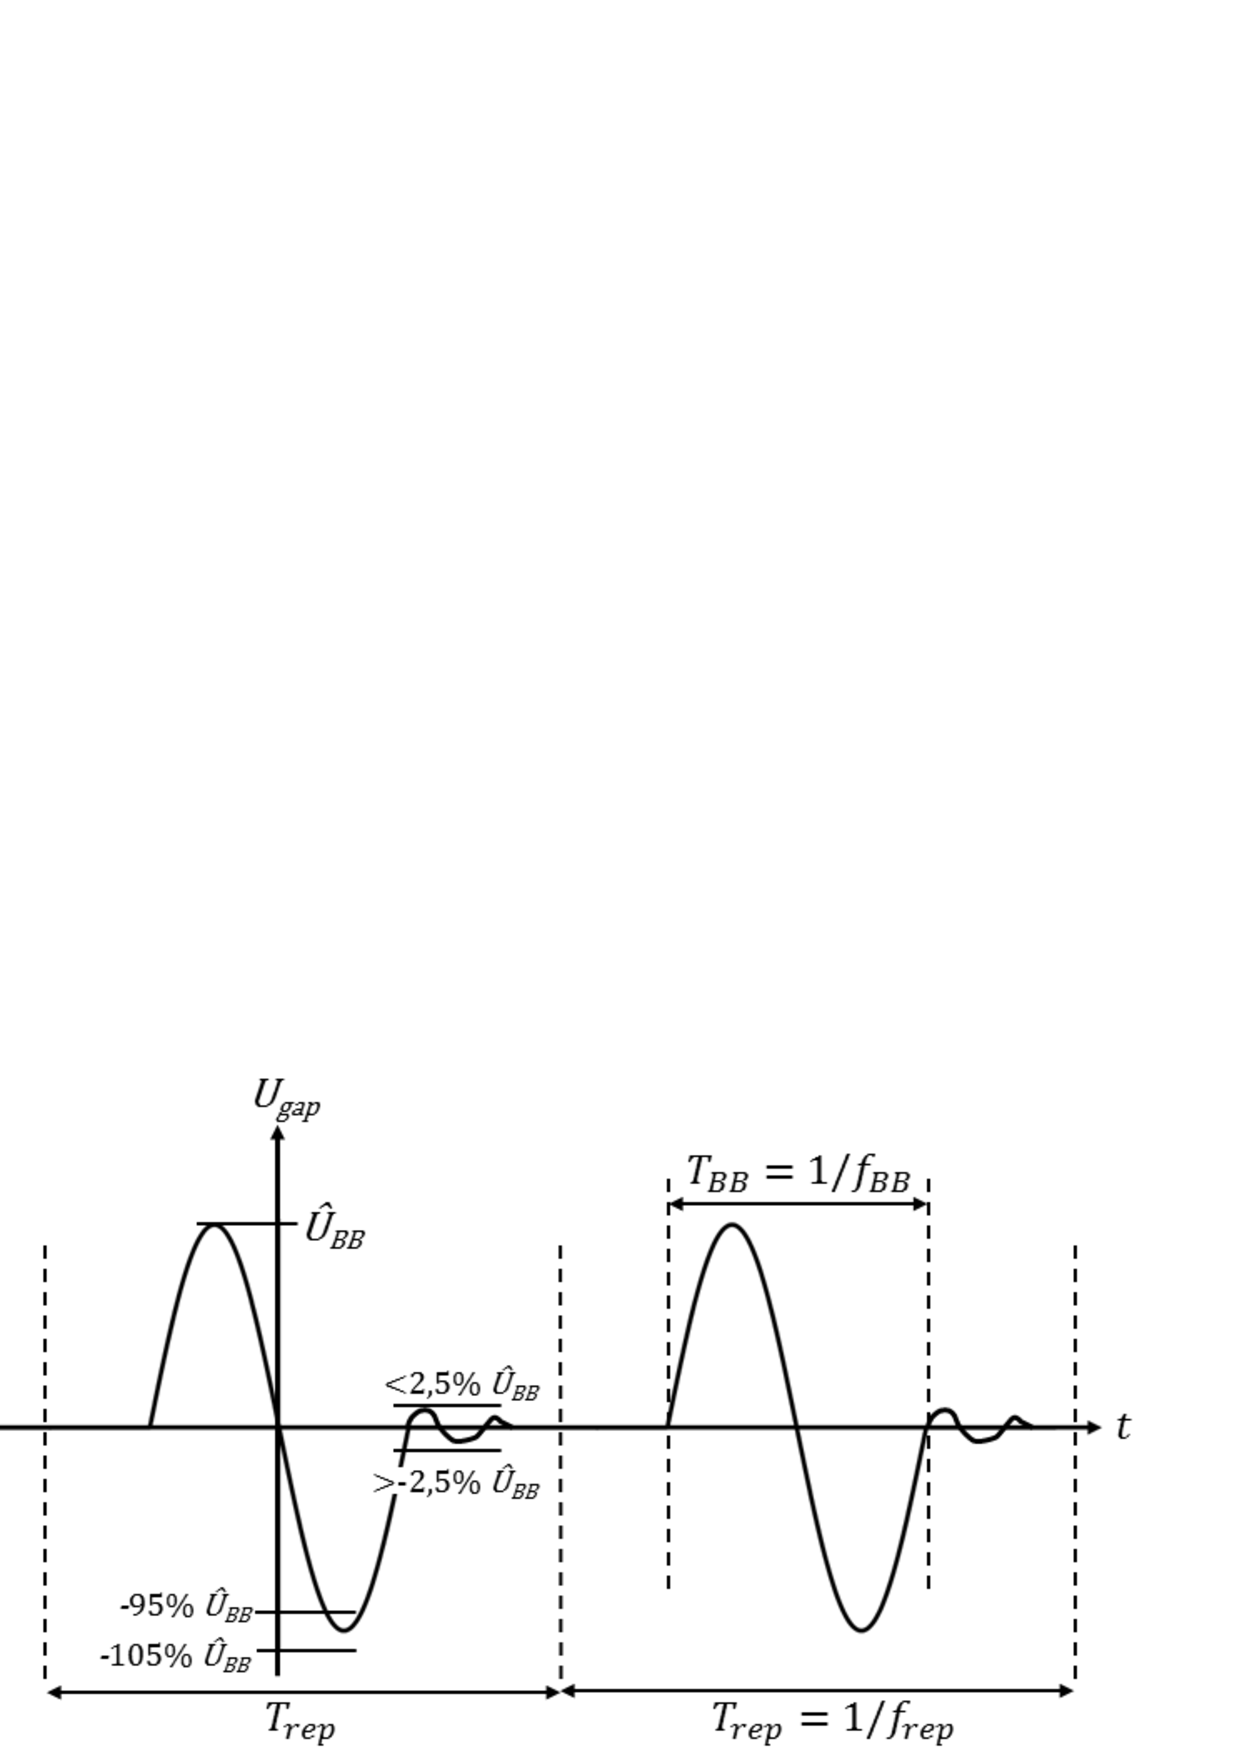
\includegraphics[width=0.7\textwidth]{eps/BB_req.pdf}
  \caption{Ausgangssignal}
  \label{fig:BB_req}
\end{figure}

Dabei benutzen wir im Folgenden $f_{rep}$ für die Wiederholfrequenz des Spannungssignals und die Barrier Bucket Frequenz $f_{BB}$ bestimmt die Breite der Potential Barriere. Für unsere Messungen haben wir ${f_{rep} = 900 \si{\kilo \hertz}}$ und ${f_{BB} = 5 \si{\mega \hertz}}$ verwendet.


\section[Modell und Konvention]{Versuchsaufbau und Modell}
\label{sec:einf.modell_BB}
Der Prototyp des ESR BB besteht aus einem Funktionsgenerator (Keysight 3600A series 2-channel AWG), einem Verstärker (AR1000A225) und der Breitband Ringkern Kavität. Der Versuchsaufbau ist in \figref{fig:Aufbau} gezeigt.\\Dabei kann angenommen werden, dass sich das System bis $\hat{U}_{BB} = 550V$ annähernd linear verhält und durch die Übertragungsfunktion $\Hcompl$ beschrieben werden kann. Eine mathematische Modellierung ist ebenfalls in \figref{fig:Aufbau} gegeben, bei der zur linearen Übertragungsfunktion $\Hcompl$ noch eine nichtlineare Kennlinie enthalten ist. Die Größen werden im nächsten Abschnitt erklärt.
\begin{figure}[H]
	\centering
	\includegraphics[width=0.7\textwidth]{eps/Aufbau.pdf}
	\caption{Versuchsaufbau und Modell}
  	\label{fig:Aufbau}
\end{figure}


\subsection{Hammerstein Modell}
\label{subsec:einf.modell_BB.hammerstein}
In \figref{fig:Hammerstein} sind alle von uns verwendeten Größen dargestellt. $U_{in}$ ist die Eingangsspannung vom Funktionsgenerator. Der erste Block in \figref{fig:Hammerstein} stellt die nichtlineare Modellierung dar. Die Spannung $U_{?}$ ist eine rein virtuelle Größe und kann wie in \ref{eq:Uquest} über die Koeffizienten $a_n$ berechnet werden. Bei der Potenzreihe hatte $N = 3$ in der MATLAB Implementierung schon gute Ergebnisse geliefert und wurde von uns auch weiterhin so verwendet. Die nichtlinearen Kennlinie im Folgenden nur noch als $K$ bezeichnet wird als Look-Up Tabelle in unserem Programm hinterlegt. Die Spannung $U_{out}$ ist die Gap Spannung in der Kavität.
\begin{figure}[H]
	\centering
	\includegraphics[width=0.5\textwidth]{eps/Hammerstein.pdf}
	\caption{Hammerstein Modell}
  	\label{fig:Hammerstein}
\end{figure}
\begin{align}
	U_?(t)=\sum_{n=1}^N \, a_n \, \left[ U_{in}(t) \right]^n
	\label{eq:Uquest}
	\qquad
	\Uout \oft = \mathscr{F}^{-1} \left\{ \Hcompl \ofomega \cdot \Uinc \ofomega \right\}
\end{align}


\section{Motivation}
\label{sec:einf.motivation}
Dieses Modell wurde bis auf die Berechnung von $K$ schon erfolgreich in Python implementiert, dabei sei auf das Projektseminar \cite{PJS_Denys} verwiesen. Deshalb lag unsere Motivation darin dieses Modell in Python zu vervollständigen, um dann eine möglichen Optimierungsansatz aufzustellen.


\section{Aufgabenstellung}
\label{sec:einf.problem}
Im Rahmen unseres Projektseminar sollte eine iterative Optimierung der Vorverzerrung auf Basis einer Hammersteinmodellierung in Python implementiert werden. Dabei sollte das Tool die nichtlineare Kennlinie $K$ und die Übertragungsfunktion $\Hcompl$ wechselseitig optimieren, wobei eine optimale Gewichtung der Parameter zur Optimierung noch nicht erreicht werden musste.
\end{document}